\rchapter{Advection Equations}

\section{Introduction}

Advection equations describe the transport of a conserved quantity. They are therefore necessary to describe the movement of particles in a plasma. The derivation of the advection equations is described in detail in chapter \ref{chapter::Gyrokinetics}.

There are many methods for solving advection equations. In this project a semi-lagrangian method will be used with Strang splitting. 

\section{Semi-Lagrangian Method}

The semi-Lagrangian method is a method of solving advection equations of the form:

\begin{equation}
 \partial_t f(\vec{x},t) + \vec{c}(\vec{x},t) \cdot \grad f(\vec{x},t) = 0
\end{equation}

As described by Garbet et al. \cite{GyrokineticSimulations}, it is a combination of the Eulerian and Lagrangian methods of solving advection equations. The Eulerian method consists of discretising the phase space on a fixed grid, and applying a grid based method such as finite differences, finite volumes, and Fourier transforms. This however leads to restrictions on the time step that can be used due to the CFL condition and can lead to dissipation.

The Lagrangian method takes advantage of the fact that advection equations arise from conservation equations to remove the restrictions on the time step. Conserved quantities are quantities whose values remain constant along a trajectory and thus obey the following rule:

\begin{align}
 &\frac{d}{dt} f(\vec{x}(t),t) &= 0\\
 &\frac{\partial}{\partial t} f(\vec{x}(t),t) + \grad f(x(t),t) \cdot \frac{\partial}{\partial t}\vec{x}(t) &= 0
\end{align}

Evidently this trajectory can therefore be described by the following equation:

\begin{equation}\label{eq::semi lagrangian trajectory definition}
 \frac{\partial}{\partial t}x(t) = c(x,t)
\end{equation}

If this equation can be solved trivially then the exact solution can be easily determined. For example, in the simplified case of a 1-D constant advection problem, the exact solution can be defined as follows:

\begin{equation}
 f(x,t) = f_0(x-ct)
\end{equation}

where $f_0(x)=f(x,0)$.

The Lagrangian method exploits these properties to create a method which does not necessarily have any restrictions on the size of the time step. Indeed the time step has no restrictions if the trajectory can be defined exactly. Otherwise it must be approximated via another method to a sufficient degree of accuracy. The method consists of following specific particles along their trajectories. These particles are chosen using statistical methods. This means that at the beginning of the simulation they should be approximately evenly spaced, however it is not guaranteed that this spacing is maintained. This can lead to areas which at a given time contain very few of the chosen particles. This means that the approximation in that area is not very precise.

The semi-Lagrangian method tries to combine the Eulerian and Lagrangian methods to benefit from the advantages of each. The method is grid-based but still uses trajectory integration. At each time step the trajectory defined by equation \ref{eq::semi lagrangian trajectory definition} is followed back from each grid point to its position at the start of the time step. The value of the function at the starting point is then approximated and the value is saved at the grid point.

There are multiple ways of approximating the value at the grid point. Here splines will be used.

\section{Strang Splitting} \label{sec::Strang}

Advection equations can be expressed as:

\begin{equation}
 \partial_t f = \sum_i L_i(f)
\end{equation}

where $L_i(f)$ is an operator. If the operators can be expressed as matrices then the exact solution can be defined as follows:

\begin{equation}
 f(t) = e^{(\sum_i L_i)t}f_0
\end{equation}

Of course in the case of an advection equation the operator is a derivative not a matrix. However, the definition of the derivative means that it can be represented as a matrix of infinite dimensions. Therefore the approximation is appropriate.

If the matrices are commutative then the solution can be expressed as:

\begin{equation}
 f(t) = \prod_i e^{L_it}f_0
\end{equation}

This means that the numerical equation can be split into multiple equations:

\begin{align}
 f(t) = e^{L_n t} f_{n-1}(t)\\
 f_i(t) = e^{L_i t} f_{i-1}(t)\\
 f_1(t) = e^{L_1 t} f_0
\end{align}

This is useful as the resulting equations are much simpler and can be solved on contiguous data sets.

However the matrices representing the derivatives are not necessarily commutative which means that the equation $e^{A+B}=e^Ae^B$ does not necessarily hold. This means that at each time step there is an error due to this supposition. In the simplest splitting method, Lie splitting, this error is $\o{\tau}$. The Strang splitting method reduces this error to $\o{\tau^2}$. The process is as follows:

\begin{enumerate}
 \item One half time step of the least expensive operators
 \item One time step of the most expensive operator
 \item One half time step of the least expensive operators
\end{enumerate}

The proof of the order of the error is given below, where operators A and B are supposed to be relatively inexpensive compared to operator C:

\begin{align*}
 &e^{A\frac{\tau}{2}}e^{B\frac{\tau}{2}}e^{C\tau}e^{B\frac{\tau}{2}}e^{A\frac{\tau}{2}}\\
 =& \left(\Id + A\frac{\tau}{2} + \frac{A^2\tau^2}{8} + \frac{A^3\tau^3}{48} + \O{\tau^4}\right)\cdot\\
 & \left(\Id + B\frac{\tau}{2} + \frac{B^2\tau^2}{8} + \frac{B^3\tau^3}{48} + \O{\tau^4}\right)\cdot\\
 & \left(\Id + C\tau + \frac{C^2\tau^2}{2} + \frac{C^3\tau^3}{6} + \O{\tau^4}\right)\cdot\\
 & \left(\Id + B\frac{\tau}{2} + \frac{B^2\tau^2}{8} + \frac{B^3\tau^3}{48} + \O{\tau^4}\right)\cdot\\
 & \left(\Id + A\frac{\tau}{2} + \frac{A^2\tau^2}{8} + \frac{A^3\tau^3}{48} + \O{\tau^4}\right)\\
 =& \Id + \left(A+B+C\right)\tau + (A+B+C)^2\frac{\tau^2}{2} + \O{\tau^3}\\
 =& e^{(A+B+C)} + \O{\tau^3}
\end{align*}

\section{Screw-Pinch model - Numerical Methods}

As explained in chapter \ref{chapter::Gyrokinetics}, the particle distribution function $f(t,r,\theta,z,v_\parallel)$ must satisfy equation \ref{eq::Continuity Cylindrical}:

\begin{equation*}
 \partial_t f + \{\phi, f \} + v_\parallel \nabla_\parallel f - \nabla_\parallel \phi\,\, \partial_{v_\parallel} f = 0
\end{equation*}

As described in section \ref{sec::Strang}, this equation can be split into multiple advection equations. These equations are:

\begin{align}
 \partial_t f + v_\parallel \nabla_\parallel f &= 0 \label{Eq::Advection1}\\
 \partial_t f + \nabla_\parallel \phi\,\, \partial_{v_{\parallel}} f &= 0 \label{Eq::Advection2}\\
 \partial_t f + \{\phi, f\} &= 0 \label{Eq::Advection3}
\end{align}

where $\{\phi,f\}$ is a Poisson bracket, defined as follows:

\begin{equation}
 \{\phi,f\}=-\frac{\partial_\theta\phi}{rB_0}\partial_r f + \frac{\partial_r\phi}{rB_0}\partial_\theta f
\end{equation}

\subsection{Flux surface advection operator}\label{Flux operator}

The flux surface advection operator defined by equation \ref{Eq::Advection1} is a two-dimensional semi-lagrangian operator. The advection coefficient has no relation to the flux surface, therefore the advection is constant on each surface and the trajectory used by the semi-lagrangian method can be defined exactly.

The value of the particle distribution function outside of the grid points is approximated using a combination of a one-dimensional cubic spline interpolation in the $\theta$ direction and a 5-th order Lagrange interpolation (field-aligned) in the z direction. The six grid points on the z-axis, nearest to the final position, are determined. The theta coordinates of the flux-aligned line which passes through the final position, are calculated at these z values. The values of the particle distribution function at these six points are then approximated using the one-dimensional cubic spline interpolation in the $\theta$ direction. The six values are finally used to construct a 5-th order Lagrange interpolation (field-aligned) in the z direction and the value at the final position is determined from this interpolation.

\subsection{V-Parallel surface advection operator}\label{V-parallel operator}

The v$_\parallel$ surface advection operator defined by equation \ref{Eq::Advection2} is a one-dimensional semi-lagrangian operator which uses a cubic spline interpolation to approximate the value of the particle distribution function outside of the grid points. The parallel gradient of phi depends only on the spatial coordinates and is therefore constant along the v$_\parallel$ surface. As a result the trajectory used by the semi-lagrangian method can be defined exactly.

The parallel gradient of phi is computed using 6th order finite differences (field-aligned) in the z direction. This is calculated as described by Latu et al. \cite{YamanPaper} using the following equation:

\begin{equation}
 \nabla_\parallel \phi(r_i,\theta_j,z_k)\approx \frac{b_z(r_i)}{\Delta z} \underset{l=-3}{\overset{3}{\sum}}w_l\tilde{\phi}\left(r_i,\text{fieldline}_\theta\left(\theta_j,\frac{z_k}{R_0},k+l\right),z_{k+l}\right)
\end{equation}

where the fieldline is defined as follows:

\begin{equation}
 \text{fieldline}_\theta(\theta^\star,\varphi^\star,j^\star+k)=\theta^\star + \iota(r_0)\left(\varphi_{j^\star+k}-\varphi^\star\right)
\end{equation}

and the weights are:

$$w_0=0,\quad w_1=-w_{-1}=\frac{3}{4},\quad w_2=-w_{-2}=-\frac{3}{20},\quad w_3=-w_{-3}=\frac{1}{60}$$

\subsection{Poloidal surface advection operator}\label{Poloidal operator}

The poloidal surface advection equation as defined by equation \ref{Eq::Advection3} can be rewritten as follows:

\begin{equation}\label{Eq::Poloidal operator}
 \partial_t f -\frac{\partial_\theta\phi}{rB_0}\partial_r f + \frac{\partial_r\phi}{rB_0}\partial_\theta f = 0
\end{equation}

The operator used is a two-dimensional semi-lagrangian operator which uses a 2-D tensor-product cubic spline interpolation in the ($r,\theta$) plane to approximate the value of the particle distribution function outside of the grid points.

The trajectory used by the semi-lagrangian operator is found using the second order Runge method. This can either be explicit or implicit. The explicit form (also known as Heun's method) is defined as follows:

\begin{equation}
 f^{n+1}=f^{n}-\frac{\tau}{2}\left(\{\phi,f^{n}\}+\{\phi,f^{n}-\tau\{\phi,f^{n}\}\right)
\end{equation}

The implicit form is an iterative method:

\begin{equation}
 f^{n+1}_{i+1}=f^{n}-\frac{\tau}{2}\left(\{\phi,f^{n}\}+\{\phi,f^{n+1}_{i}\}\right)
\end{equation}

It is considered to have converged when $\|f^{n+1}_{i+1}-f^{n+1}_{i}\|<\varepsilon$ for a given tolerance $\varepsilon$.

\subsection{Strang Splitting}

As mentioned in section \ref{sec::Strang}, expensive operators will only be used once per time-step while relatively inexpensive operators will be used twice.

\begin{table}[ht]
 \centering
 \begin{tabular}{|c|c|c|}
  \hline
  Operator & Time per step [s] & Time per grid [s]\\
  \hline
  Flux surface advection & $2.85\cdot 10^{-3}$ & 1.23\\
  \hline
  V-Parallel surface advection & $3.08\cdot 10^{-4}$ & 2.78\\
  \hline
  Poloidal surface advection & $3.41\cdot 10^{-2}$ & 12.7\\
  \hline
 \end{tabular}
 \caption{\label{tab::advection time}Time required for one time step of each advection operator averaged over 1000 steps. 20 points are used in each direction on the grid}
\end{table}

Table \ref{tab::advection time} shows the time required for one step of each operator. As the poloidal surface advection is approximately ten times more expensive than the other operators, this operator will only be used once per time step.

The algorithm is therefore:
\begin{enumerate}[noitemsep]
 \item Use the operator described in equation \ref{Eq::Advection1} with a time step of $\frac{\tau}{2}$
 \item Use the operator described in equation \ref{Eq::Advection2} with a time step of $\frac{\tau}{2}$
 \item Use the operator described in equation \ref{Eq::Advection3} with a time step of $\tau$
 \item Use the operator described in equation \ref{Eq::Advection2} with a time step of $\frac{\tau}{2}$
 \item Use the operator described in equation \ref{Eq::Advection1} with a time step of $\frac{\tau}{2}$
\end{enumerate}


\section{Convergence}

\subsection{V-Parallel surface advection}

The v$_\parallel$ surface advection operator defined by equation \ref{Eq::Advection2} can be written more simply as follows:

\begin{equation}
 \partial_t f(v_\parallel) + c \partial_{v_\parallel}f = 0
\end{equation}

this formulation allows us to test the advection operator alone.

As the trajectory for the v-parallel surface advection can be calculated exactly, the convergence order ought to be equal to the order of the spline approximation. Here the function will be approximated by 3rd degree splines.

The convergence is tested using the following function:
\begin{equation}\label{eq::v parallel init}
 f_0(v_\parallel) = \cos(0.1 \pi v_\parallel)^4
\end{equation}
over the domain $\Omega=[-5,5]$. The boundary conditions are such that $f_0(\reel\backslash\Omega)=0$

This function is chosen as on the boundary $\delta\Omega$, $f_0(\delta\Omega)=f_0'(\delta\Omega)=f_0''(\delta\Omega)=f_0'''(\delta\Omega)=0$. This is important as it ensures that the spline approximation is $\mathcal{C}^3$ at the boundary.

\begin{table}[ht]
\centering
 \begin{tabular}{|r c|c|c|c|c|}
  \hline
  \bf N$_x$ & & \bf L$^2$ norm       & \bf Order & \bf L$^\infty$ norm  & \bf Order\\
  \hline
  64     & & $ 1.49 \cdot 10^{ -5 }$ &       & $ 8.52 \cdot 10^{ -6 }$ &  \\
  \hline
  128     & & $ 1.63 \cdot 10^{ -6 }$ &  3.20  & $ 9.36 \cdot 10^{ -7 }$ &  3.19  \\
  \hline
  256     & & $ 1.94 \cdot 10^{ -7 }$ &  3.07  & $ 1.12 \cdot 10^{ -7 }$ &  3.06  \\
  \hline
  512     & & $ 2.39 \cdot 10^{ -8 }$ &  3.02  & $ 1.38 \cdot 10^{ -8 }$ &  3.02  \\
  \hline
  1024     & & $ 2.97 \cdot 10^{ -9 }$ &  3.01  & $ 1.71 \cdot 10^{ -9 }$ &  3.01  \\
  \hline
  2048     & & $ 3.69 \cdot 10^{ -10 }$ &  3.01  & $ 2.12 \cdot 10^{ -10 }$ &  3.01  \\
  \hline
  4096     & & $ 4.60 \cdot 10^{ -11 }$ &  3.01  & $ 2.67 \cdot 10^{ -11 }$ &  2.99  \\
  \hline
 \end{tabular}
 \caption{\label{V Parallel convergence} v$_\parallel$ advection with c = 2, $N_x\cdot dt$ = 0.32, endTime = 1s, with initial conditions described by equation \ref{eq::v parallel init}}
\end{table}

The results can be seen in table \ref{V Parallel convergence}. We see that the convergence is of 3-rd order as expected.

The convergence of the parallel gradient of phi is tested using the following equation:
\begin{equation}
 \phi(\theta,z)= \cos(\theta)^2 + \sin(0.1\pi z)^2
\end{equation}

The result should therefore be the following:
\begin{equation}
 \grad_\parallel\phi(\theta,z) = 0.2\pi b_z\sin(0.1\pi z)\cos(0.1\pi z) - 2 b_\theta \cos(\theta)\sin(\theta)
\end{equation}

\begin{table}[ht]
\centering
 \begin{tabular}{|r c|c|c|c|c|}
  \hline
  \bf N$_z$ & & \bf L$^2$ norm       & \bf Order & \bf L$^\infty$ norm  & \bf Order\\
  \hline
  8  & & $ 1.80 \cdot 10^{ -1 }$ &       & $ 2.08 \cdot 10^{ -2 }$ &        \\
  \hline
  16  & & $ 3.00 \cdot 10^{ -3 }$ &  5.91  & $ 4.67 \cdot 10^{ -4 }$ &  5.48  \\
  \hline
  32  & & $ 3.68 \cdot 10^{ -5 }$ &  6.35  & $ 7.99 \cdot 10^{ -6 }$ &  5.87  \\
  \hline
  64  & & $ 4.17 \cdot 10^{ -7 }$ &  6.46  & $ 1.28 \cdot 10^{ -7 }$ &  5.97  \\
  \hline
  128  & & $ 4.63 \cdot 10^{ -9 }$ &  6.49  & $ 2.01 \cdot 10^{ -9 }$ &  5.99  \\
  \hline
  256  & & $ 5.12 \cdot 10^{ -11 }$ &  6.50  & $ 3.18 \cdot 10^{ -11 }$ &  5.98  \\
  \hline
  512  & & $ 7.50 \cdot 10^{ -13 }$ &  6.09  & $ 9.43 \cdot 10^{ -13 }$ &  5.08  \\
  \hline
 \end{tabular}
 \caption{\label{dPhi convergence z} derivative of phi with $N_\theta$ = 1024}
\end{table}

The convergence order is tested in both the $\theta$ and $z$ directions. In the $\theta$ direction, the convergence should be due to the spline and should therefore be of order p+1 where p is the order of the spline. In the tests third order splines are used. Table \ref{dPhi convergence theta} shows that the convergence is similar to what is expected. In the $z$ direction the convergence should be of the same order as the finite differences method used (6th order). Table \ref{dPhi convergence z} shows that this is indeed the case. Both the $L_2$ and $L_\infty$ norms converge to 6th order. The $L_\infty$ norm shows one erroneous result for $N_z=512$ however this is probably due to the fact that the results approach machine precision at this point.

\begin{table}[ht]
\centering
 \begin{tabular}{|r c|c|c|c|c|}
  \hline
  \bf N$_\theta$ & & \bf L$^2$ norm       & \bf Order & \bf L$^\infty$ norm  & \bf Order\\
  \hline
  8  & & $ 1.01 \cdot 10^{ -5 }$ &       & $ 1.50 \cdot 10^{ -4 }$ &        \\
  \hline
  16  & & $ 7.62 \cdot 10^{ -7 }$ &  3.74  & $ 7.59 \cdot 10^{ -6 }$ &  4.31  \\
  \hline
  32  & & $ 6.46 \cdot 10^{ -8 }$ &  3.56  & $ 4.49 \cdot 10^{ -7 }$ &  4.08  \\
  \hline
  64  & & $ 5.65 \cdot 10^{ -9 }$ &  3.52  & $ 2.77 \cdot 10^{ -8 }$ &  4.02  \\
  \hline
  128  & & $ 4.98 \cdot 10^{ -10 }$ &  3.50  & $ 1.72 \cdot 10^{ -9 }$ &  4.00  \\
  \hline
  256  & & $ 4.39 \cdot 10^{ -11 }$ &  3.50  & $ 1.08 \cdot 10^{ -10 }$ &  4.00  \\
  \hline
  512  & & $ 3.89 \cdot 10^{ -12 }$ &  3.50  & $ 6.79 \cdot 10^{ -12 }$ &  3.99  \\
  \hline
 \end{tabular}
 \caption{\label{dPhi convergence theta} derivative of phi with $N_z$ = 1024}
\end{table}

\subsection{Poloidal advection}

The poloidal advection operator as described in section \ref{Poloidal operator} should be tested using a self-consistent potential $\phi$ such that the exact trajectory can be found and defined simply but which is sufficiently complex for a second order scheme to be required. In addition the boundary conditions must be periodic in the $\theta$ direction.

The chosen function is the following:

\begin{equation}
 \phi(r,\theta) = -5 r^2 + \sin(\theta)
\end{equation}

Using equation \ref{Eq::Poloidal operator}, the trajectory can be described by the following equations:

\begin{align*}
 \frac{\partial}{\partial t} r(t) &= - \frac{\partial_\theta\phi}{rB_0} &&= - \frac{\cos(\theta)}{rB_0}\\
 \frac{\partial}{\partial t} \theta(t) &= \frac{\partial_r\phi}{rB_0} &&= \frac{-10 r}{rB_0} = -\frac{10}{B_0}
\end{align*}

From this, it is trivial to find the explicit expression which describes the coordinate $\theta$:

\begin{equation}
 \theta(t) = \theta_0 - \frac{10}{B_0} t
\end{equation}

The expression which describes the coordinate $r$ is slightly more complicated but can also be simply determined:

\begin{align*}
 \frac{\partial}{\partial t} r(t) &= - \frac{\cos\left(\theta_0 - \frac{10}{B_0} t\right)}{rB_0}\\
 \int \frac{\partial}{\partial t}\left(\frac{1}{2}r(t)^2\right) dt &= - \frac{1}{B_0} \int \cos\left(\theta_0 - \frac{10}{B_0} t\right) dt\\
 r(t)^2 &= \frac{2}{B_0} \sin\left(\theta_0 - \frac{10}{B_0}t\right)\frac{B_0}{10} + C\\
 r(t) &= \sqrt{\frac{1}{5}\sin\left(\theta_0 - \frac{10}{B_0}t\right) + C}
\end{align*}

The initial conditions can then be used to define the unknown quantities

\begin{align}
 r(0) = r_0 &= \sqrt{\frac{1}{5}\sin(\theta_0) + C}\nonumber\\
 C &= r_0^2-\frac{1}{5}\sin(\theta_0)\nonumber\\
 r(t) &= \sqrt{\frac{1}{5}\left(\sin\left(\theta_0 - \frac{10}{B_0}t\right)-\sin(\theta_0)\right)+r_0^2}
\end{align}

The trajectories can therefore be used to find the exact solution which is used to determine the error for the convergence studies.

\begin{figure}[ht]
\centering
\begin{subfigure}[t]{.45\textwidth}
  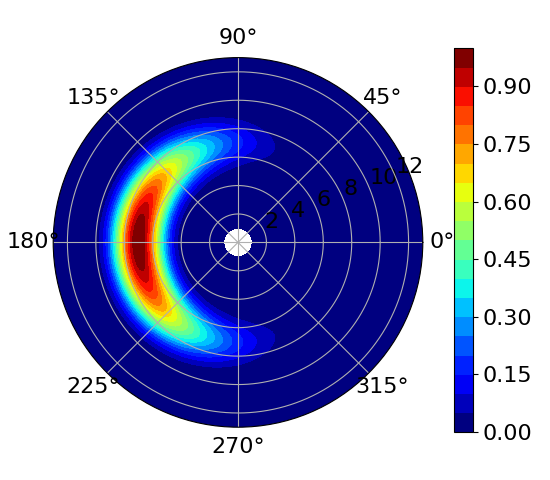
\includegraphics[width=\textwidth]{Figs/initConvergenceConds/Poloidal1}
  \caption{\label{fig::init Poloidal 1}Equation \ref{eq::poloidal init 1}}
 \end{subfigure}
 \hspace{.05\textwidth}
 \begin{subfigure}[t]{.45\textwidth}
  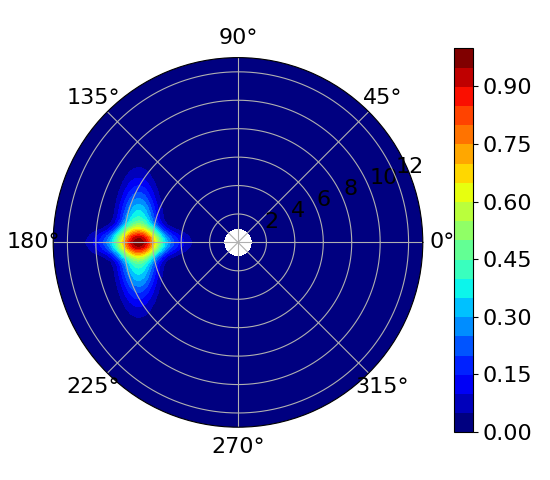
\includegraphics[width=\textwidth]{Figs/initConvergenceConds/Poloidal2}
  \caption{\label{fig::init Poloidal 2}Equation \ref{eq::poloidal init 2}}
 \end{subfigure}
 \caption{\label{fig::init conds poloidal}Initial conditions $f_0$ for the poloidal advection convergence tests as described by equations \ref{eq::poloidal init 1} and \ref{eq::poloidal init 2}}
\end{figure}


Two different initial conditions will be used. The first will be an ellipsis in the coordinates ($r$,$\theta$). The second will not be dependent on the coordinates and will have a more irregular shape as shown in figure \ref{fig::init conds poloidal}. The conditions are defined as follows:
\begin{align}
 f_0(r,\theta)&=B(r_1(r,\theta),a_1) \label{eq::poloidal init 1}\\
 f_0(r,\theta)&=B(r_2(r\cos(\theta),r\sin(\theta),a_2)+B(r_3(r\cos(\theta),r\sin(\theta)),a_2) \label{eq::poloidal init 2}\\
 B(r,a) &= 
 \begin{cases}
  \cos\left(\frac{\pi r}{2 a}\right)^4\quad\quad \text{ if }r\leq a\\
  0\quad\quad\quad \text{otherwise}
 \end{cases}\nonumber\\
r_1(x,y) &= \sqrt{(x-7)^2+2*(y-\pi)^2}\nonumber\\
r_2(x,y) &= \sqrt{(x+7)^2+8*y^2}\nonumber\\
r_3(x,y) &= \sqrt{4*(x+7)^2+0.5*y^2}\nonumber\\
a_1 &= 4\nonumber\\
a_2 &= 6\nonumber
\end{align}
over the domain $\Omega=[0,20]\cross[0,2\pi]$. The boundary conditions are periodic in $\theta$ and such that $f_0(\reel\backslash\Omega)=0$.

\begin{table}[ht]
\centering
 \begin{tabular}{|r c|r c|c|c|c|c|}
  \hline
  \multicolumn{2}{|c|}{\bf N$_x$} & \multicolumn{2}{|c|}{\bf N$_y$} & \bf L$^2$ norm       & \bf Order & \bf L$^\infty$ norm  & \bf Order\\
  \hline
  \hline
  32  & &  32     & & $ 1.79 \cdot 10^{ -3 }$ &       & $ 3.05 \cdot 10^{ -4 }$ &  \\
  \hline
  64  & &  64     & & $ 2.19 \cdot 10^{ -4 }$ &  3.03  & $ 3.71 \cdot 10^{ -5 }$ &  3.04  \\
  \hline
  128  & &  128     & & $ 2.72 \cdot 10^{ -5 }$ &  3.00  & $ 4.61 \cdot 10^{ -6 }$ &  3.01  \\
  \hline
  256  & &  256     & & $ 3.41 \cdot 10^{ -6 }$ &  3.00  & $ 5.75 \cdot 10^{ -7 }$ &  3.00  \\
  \hline
  512  & &  512     & & $ 4.26 \cdot 10^{ -7 }$ &  3.00  & $ 7.19 \cdot 10^{ -8 }$ &  3.00  \\
  \hline
 \end{tabular}
 \caption{\label{Poloidal dx convergence eq1} Spatial convergence for poloidal advection, $N_x\cdot dt = 0.032$ s, $t_{\text{end}}$=0.2s, $f_0$ is given by equation \ref{eq::poloidal init 1}}
\end{table}

\begin{table}[ht]
\centering
 \begin{tabular}{|r c|r c|c|c|c|c|}
  \hline
  \multicolumn{2}{|c|}{\bf N$_x$} & \multicolumn{2}{|c|}{\bf N$_y$} & \bf L$^2$ norm       & \bf Order & \bf L$^\infty$ norm  & \bf Order\\
  \hline
  \hline
  32  & &  32     & & $ 2.01 \cdot 10^{ -1 }$ &       & $ 6.00 \cdot 10^{ -2 }$ &  \\
  \hline
  64  & &  64     & & $ 1.32 \cdot 10^{ -1 }$ &  0.61  & $ 6.34 \cdot 10^{ -2 }$ &  -0.08  \\
  \hline
  128  & &  128     & & $ 1.99 \cdot 10^{ -2 }$ &  2.73  & $ 9.89 \cdot 10^{ -3 }$ &  2.68  \\
  \hline
  256  & &  256     & & $ 2.22 \cdot 10^{ -3 }$ &  3.17  & $ 1.03 \cdot 10^{ -3 }$ &  3.27  \\
  \hline
  512  & &  512     & & $ 2.60 \cdot 10^{ -4 }$ &  3.09  & $ 1.23 \cdot 10^{ -4 }$ &  3.06  \\
  \hline
  1024 & & 1024     & & $ 3.20 \cdot 10^{ -5 }$ &  3.03 & $ 1.51 \cdot 10^{ -5 }$ & 3.02 \\
  \hline
 \end{tabular}
 \caption{\label{Poloidal dx convergence eq2} Spatial convergence for poloidal advection, $N_x\cdot dt = 0.032$ s, $t_{\text{end}}$=0.05s, $f_0$ is given by equation \ref{eq::poloidal init 2}}
\end{table}

To determine the order of convergence the spatial and temporal convergence orders must be treated separately. In order to  determine the spatial convergence the calculated trajectory is used instead of the second order scheme. This means that all errors are due to the interpolation. As a result the convergence order ought to be equal to the order of the spline approximation. Here the function will be approximated by 3rd degree splines.

Tables \ref{Poloidal dx convergence eq1} and \ref{Poloidal dx convergence eq2} confirm this convergence order. Although it should be noted that shapes which are not dependent on the coordinate system require more points in order to achieve a given accuracy and convergence is only seen once the error is sufficiently small.

In order to determine the temporal convergence order a large number of spatial points is used to ensure that the error is dominated by the errors due to the trajectory calculation. The convergence should therefore be second order. This is confirmed by table \ref{Poloidal dt convergence}

\begin{table}[ht]
\centering
 \begin{tabular}{|r c|l|c|c|c|c|}
  \hline
  \multicolumn{2}{|c|}{\bf N$_t$} & \multicolumn{1}{|c|}{\bf dt} & \bf L$^2$ norm       & \bf Order & \bf L$^\infty$ norm  & \bf Order\\
  \hline
  10  & &  0.1     & $ 3.81 \cdot 10^{ -3 }$ &       & $ 9.19 \cdot 10^{ -4 }$ &  \\
  \hline
  20  & &  0.05     & $ 9.43 \cdot 10^{ -4 }$ &  2.01  & $ 2.28 \cdot 10^{ -4 }$ &  2.01  \\
  \hline
  40  & &  0.025     & $ 2.35 \cdot 10^{ -4 }$ &  2.00  & $ 5.71 \cdot 10^{ -5 }$ &  2.00  \\
  \hline
  80  & &  0.0125     & $ 5.88 \cdot 10^{ -5 }$ &  2.00  & $ 1.43 \cdot 10^{ -5 }$ &  2.00  \\
  \hline
  160  & &  0.00625   & $ 1.47 \cdot 10^{ -5 }$ &  2.00  & $ 3.57 \cdot 10^{ -6 }$ &  2.00  \\
  \hline
 \end{tabular}
 \caption{\label{Poloidal dt convergence} Temporal convergence for poloidal advection, with N$_x$ = N$_y$ = 100, endTime = 1s, $f_0$ is given by equation \ref{eq::poloidal init 1}}
\end{table}

\subsection{Flux-surface advection}

The flux-surface advection operator is defined by equation \ref{Eq::Advection1}:

\begin{equation}
 \partial_t f(v_\parallel) + c \grad_\parallel f = 0
\end{equation}

As the trajectory for the flux-surface advection can be calculated exactly, the convergence order ought to depend on a combination of the error due to the spline approximation and the error due to the Lagrange interpolation. A combination of different ordered convergences can be difficult to identify. Therefore for the purpose of the tests a 3-rd degree Lagrange interpolation will be used in place of the 5-th order interpolation. The function will still be approximated by 3rd degree splines. The convergence therefore ought to be of 3-rd order.

The convergence is tested using the following function:
\begin{align}
 f_0(\theta,z)&=B(r_1(r,\theta),a_1) \label{eq::flux init}\\
 B(r,a) &= 
 \begin{cases}
  \cos\left(\frac{\pi r}{2 a}\right)^4\quad\quad \text{ if }r\leq a\\
  0\quad\quad\quad \text{otherwise}
 \end{cases}\nonumber\\
 r_1(x,y) &= \sqrt{(x-10)^2+2*(y-\pi)^2}\nonumber\\
 a_1 &= 4\nonumber
\end{align}
over the domain $\Omega=[0,2\pi]\cross[0,20]$. The boundary conditions are periodic in $\theta$ and such that $f_0(\reel\backslash\Omega)=0$.

This function is chosen as it is $\mathcal{C}^3$ everywhere.

\begin{table}[ht]
\centering
 \begin{tabular}{|r c|r c|l c|c|c|c|c|}
  \hline
  \multicolumn{2}{|c|}{\bf N$_\theta$} & \multicolumn{2}{|c|}{\bf N$_z$} & \multicolumn{2}{|c|}{\bf dt} & \bf L$^2$ norm       & \bf Order & \bf L$^\infty$ norm  & \bf Order\\
  \hline
  32  & &  32  & &  0.1     & & $ 8.26 \cdot 10^{ -2 }$ &       & $ 4.96 \cdot 10^{ -2 }$ &  \\
  \hline
  64  & &  64  & &  0.05     & & $ 1.29 \cdot 10^{ -2 }$ &  2.67  & $ 7.97 \cdot 10^{ -3 }$ &  2.64  \\
  \hline
  128  & &  128  & &  0.025     & & $ 1.70 \cdot 10^{ -3 }$ &  2.93  & $ 1.08 \cdot 10^{ -3 }$ &  2.88  \\
  \hline
  256  & &  256  & &  0.0125     & & $ 2.14 \cdot 10^{ -4 }$ &  2.99  & $ 1.36 \cdot 10^{ -4 }$ &  2.99  \\
  \hline
  512  & &  512  & &  0.00625     & & $ 2.68 \cdot 10^{ -5 }$ &  3.00  & $ 1.71 \cdot 10^{ -5 }$ &  3.00  \\
  \hline
 \end{tabular}
 \caption{\label{Flux dx convergence} Spatial convergence for the flux advection operator with $t_{\text{end}}$ = 1s, $f_0$ as given by equation \ref{eq::flux init}, 3rd degree Lagrange interpolation}
\end{table}

The results can be seen in table \ref{V Parallel convergence}. We see that the convergence is of 3-rd order as expected.